%% bare_conf_compsoc.tex
%% V1.4b
%% 2015/08/26
%% by Michael Shell
%% See:
%% http://www.michaelshell.org/
%% for current contact information.
%%
%% This is a skeleton file demonstrating the use of IEEEtran.cls
%% (requires IEEEtran.cls version 1.8b or later) with an IEEE Computer
%% Society conference paper.
%%
%% Support sites:
%% http://www.michaelshell.org/tex/ieeetran/
%% http://www.ctan.org/pkg/ieeetran
%% and
%% http://www.ieee.org/

%%*************************************************************************
%% Legal Notice:
%% This code is offered as-is without any warranty either expressed or
%% implied; without even the implied warranty of MERCHANTABILITY or
%% FITNESS FOR A PARTICULAR PURPOSE! 
%% User assumes all risk.
%% In no event shall the IEEE or any contributor to this code be liable for
%% any damages or losses, including, but not limited to, incidental,
%% consequential, or any other damages, resulting from the use or misuse
%% of any information contained here.
%%
%% All comments are the opinions of their respective authors and are not
%% necessarily endorsed by the IEEE.
%%
%% This work is distributed under the LaTeX Project Public License (LPPL)
%% ( http://www.latex-project.org/ ) version 1.3, and may be freely used,
%% distributed and modified. A copy of the LPPL, version 1.3, is included
%% in the base LaTeX documentation of all distributions of LaTeX released
%% 2003/12/01 or later.
%% Retain all contribution notices and credits.
%% ** Modified files should be clearly indicated as such, including  **
%% ** renaming them and changing author support contact information. **
%%*****************x********************************************************


% *** Authors should verify (and, if needed, correct) their LaTeX system  ***
% *** with the testflow diagnostic prior to trusting their LaTeX platform ***
% *** with production work. The IEEE's font choices and paper sizes can   ***
% *** trigger bugs that do not appear when using other class files.       ***                          ***
% The testflow support page is at:
% http://www.michaelshell.org/tex/testflow/



\documentclass[conference,compsoc]{IEEEtran}
% Some/most Computer Society conferences require the compsoc mode option,
% but others may want the standard conference format.
%
% If IEEEtran.cls has not been installed into the LaTeX system files,
% manually specify the path to it like:
% \documentclass[conference,compsoc]{../sty/IEEEtran}





% Some very useful LaTeX packages include:
% (uncomment the ones you want to load)


% *** MISC UTILITY PACKAGES ***
%
%\usepackage{ifpdf}
% Heiko Oberdiek's ifpdf.sty is very useful if you need conditional
% compilation based on whether the output is pdf or dvi.
% usage:
% \ifpdf
%   % pdf code
% \else
%   % dvi code
% \fi
% The latest version of ifpdf.sty can be obtained from:
% http://www.ctan.org/pkg/ifpdf
% Also, note that IEEEtran.cls V1.7 and later provides a builtin
% \ifCLASSINFOpdf conditional that works the same way.
% When switching from latex to pdflatex and vice-versa, the compiler may
% have to be run twice to clear warning/error messages.






% *** CITATION PACKAGES ***
%
\ifCLASSOPTIONcompsoc
  % IEEE Computer Society needs nocompress option
  % requires cite.sty v4.0 or later (November 2003)
  \usepackage[nocompress]{cite}
\else
  % normal IEEE
  \usepackage{cite}
\fi
% cite.sty was written by Donald Arseneau
% V1.6 and later of IEEEtran pre-defines the format of the cite.sty package
% \cite{} output to follow that of the IEEE. Loading the cite package will
% result in citation numbers being automatically sorted and properly
% "compressed/ranged". e.g., [1], [9], [2], [7], [5], [6] without using
% cite.sty will become [1], [2], [5]--[7], [9] using cite.sty. cite.sty's
% \cite will automatically add leading space, if needed. Use cite.sty's
% noadjust option (cite.sty V3.8 and later) if you want to turn this off
% such as if a citation ever needs to be enclosed in parenthesis.
% cite.sty is already installed on most LaTeX systems. Be sure and use
% version 5.0 (2009-03-20) and later if using hyperref.sty.
% The latest version can be obtained at:
% http://www.ctan.org/pkg/cite
% The documentation is contained in the cite.sty file itself.
%
% Note that some packages require special options to format as the Computer
% Society requires. In particular, Computer Society  papers do not use
% compressed citation ranges as is done in typical IEEE papers
% (e.g., [1]-[4]). Instead, they list every citation separately in order
% (e.g., [1], [2], [3], [4]). To get the latter we need to load the cite
% package with the nocompress option which is supported by cite.sty v4.0
% and later.





% *** GRAPHICS RELATED PACKAGES ***
%
\ifCLASSINFOpdf
  % \usepackage[pdftex]{graphicx}
  % declare the path(s) where your graphic files are
  % \graphicspath{{../pdf/}{../jpeg/}}
  % and their extensions so you won't have to specify these with
  % every instance of \includegraphics
  % \DeclareGraphicsExtensions{.pdf,.jpeg,.png}
\else
  % or other class option (dvipsone, dvipdf, if not using dvips). graphicx
  % will default to the driver specified in the system graphics.cfg if no
  % driver is specified.
  % \usepackage[dvips]{graphicx}
  % declare the path(s) where your graphic files are
  % \graphicspath{{../eps/}}
  % and their extensions so you won't have to specify these with
  % every instance of \includegraphics
  % \DeclareGraphicsExtensions{.eps}
\fi
% graphicx was written by David Carlisle and Sebastian Rahtz. It is
% required if you want graphics, photos, etc. graphicx.sty is already
% installed on most LaTeX systems. The latest version and documentation
% can be obtained at: 
% http://www.ctan.org/pkg/graphicx
% Another good source of documentation is "Using Imported Graphics in
% LaTeX2e" by Keith Reckdahl which can be found at:
% http://www.ctan.org/pkg/epslatex
%
% latex, and pdflatex in dvi mode, support graphics in encapsulated
% postscript (.eps) format. pdflatex in pdf mode supports graphics
% in .pdf, .jpeg, .png and .mps (metapost) formats. Users should ensure
% that all non-photo figures use a vector format (.eps, .pdf, .mps) and
% not a bitmapped formats (.jpeg, .png). The IEEE frowns on bitmapped formats
% which can result in "jaggedy"/blurry rendering of lines and letters as
% well as large increases in file sizes.
%
% You can find documentation about the pdfTeX application at:
% http://www.tug.org/applications/pdftex





% *** MATH PACKAGES ***
%
%\usepackage{amsmath}
% A popular package from the American Mathematical Society that provides
% many useful and powerful commands for dealing with mathematics.
%
% Note that the amsmath package sets \interdisplaylinepenalty to 10000
% thus preventing page breaks from occurring within multiline equations. Use:
%\interdisplaylinepenalty=2500
% after loading amsmath to restore such page breaks as IEEEtran.cls normally
% does. amsmath.sty is already installed on most LaTeX systems. The latest
% version and documentation can be obtained at:
% http://www.ctan.org/pkg/amsmath





% *** SPECIALIZED LIST PACKAGES ***
%
%\usepackage{algorithmic}
% algorithmic.sty was written by Peter Williams and Rogerio Brito.
% This package provides an algorithmic environment fo describing algorithms.
% You can use the algorithmic environment in-text or within a figure
% environment to provide for a floating algorithm. Do NOT use the algorithm
% floating environment provided by algorithm.sty (by the same authors) or
% algorithm2e.sty (by Christophe Fiorio) as the IEEE does not use dedicated
% algorithm float types and packages that provide these will not provide
% correct IEEE style captions. The latest version and documentation of
% algorithmic.sty can be obtained at:
% http://www.ctan.org/pkg/algorithms
% Also of interest may be the (relatively newer and more customizable)
% algorithmicx.sty package by Szasz Janos:
% http://www.ctan.org/pkg/algorithmicx




% *** ALIGNMENT PACKAGES ***
%
%\usepackage{array}
% Frank Mittelbach's and David Carlisle's array.sty patches and improves
% the standard LaTeX2e array and tabular environments to provide better
% appearance and additional user controls. As the default LaTeX2e table
% generation code is lacking to the point of almost being broken with
% respect to the quality of the end results, all users are strongly
% advised to use an enhanced (at the very least that provided by array.sty)
% set of table tools. array.sty is already installed on most systems. The
% latest version and documentation can be obtained at:
% http://www.ctan.org/pkg/array


% IEEEtran contains the IEEEeqnarray family of commands that can be used to
% generate multiline equations as well as matrices, tables, etc., of high
% quality.




% *** SUBFIGURE PACKAGES ***
%\ifCLASSOPTIONcompsoc
%  \usepackage[caption=false,font=footnotesize,labelfont=sf,textfont=sf]{subfig}
%\else
%  \usepackage[caption=false,font=footnotesize]{subfig}
%\fi
% subfig.sty, written by Steven Douglas Cochran, is the modern replacement
% for subfigure.sty, the latter of which is no longer maintained and is
% incompatible with some LaTeX packages including fixltx2e. However,
% subfig.sty requires and automatically loads Axel Sommerfeldt's caption.sty
% which will override IEEEtran.cls' handling of captions and this will result
% in non-IEEE style figure/table captions. To prevent this problem, be sure
% and invoke subfig.sty's "caption=false" package option (available since
% subfig.sty version 1.3, 2005/06/28) as this is will preserve IEEEtran.cls
% handling of captions.
% Note that the Computer Society format requires a sans serif font rather
% than the serif font used in traditional IEEE formatting and thus the need
% to invoke different subfig.sty package options depending on whether
% compsoc mode has been enabled.
%
% The latest version and documentation of subfig.sty can be obtained at:
% http://www.ctan.org/pkg/subfig




% *** FLOAT PACKAGES ***
%
%\usepackage{fixltx2e}
% fixltx2e, the successor to the earlier fix2col.sty, was written by
% Frank Mittelbach and David Carlisle. This package corrects a few problems
% in the LaTeX2e kernel, the most notable of which is that in current
% LaTeX2e releases, the ordering of single and double column floats is not
% guaranteed to be preserved. Thus, an unpatched LaTeX2e can allow a
% single column figure to be placed prior to an earlier double column
% figure.
% Be aware that LaTeX2e kernels dated 2015 and later have fixltx2e.sty's
% corrections already built into the system in which case a warning will
% be issued if an attempt is made to load fixltx2e.sty as it is no longer
% needed.
% The latest version and documentation can be found at:
% http://www.ctan.org/pkg/fixltx2e


%\usepackage{stfloats}
% stfloats.sty was written by Sigitas Tolusis. This package gives LaTeX2e
% the ability to do double column floats at the bottom of the page as well
% as the top. (e.g., "\begin{figure*}[!b]" is not normally possible in
% LaTeX2e). It also provides a command:
%\fnbelowfloat
% to enable the placement of footnotes below bottom floats (the standard
% LaTeX2e kernel puts them above bottom floats). This is an invasive package
% which rewrites many portions of the LaTeX2e float routines. It may not work
% with other packages that modify the LaTeX2e float routines. The latest
% version and documentation can be obtained at:
% http://www.ctan.org/pkg/stfloats
% Do not use the stfloats baselinefloat ability as the IEEE does not allow
% \baselineskip to stretch. Authors submitting work to the IEEE should note
% that the IEEE rarely uses double column equations and that authors should try
% to avoid such use. Do not be tempted to use the cuted.sty or midfloat.sty
% packages (also by Sigitas Tolusis) as the IEEE does not format its papers in
% such ways.
% Do not attempt to use stfloats with fixltx2e as they are incompatible.
% Instead, use Morten Hogholm'a dblfloatfix which combines the features
% of both fixltx2e and stfloats:
%
% \usepackage{dblfloatfix}
% The latest version can be found at:
% http://www.ctan.org/pkg/dblfloatfix




% *** PDF, URL AND HYPERLINK PACKAGES ***
%
%\usepackage{url}
% url.sty was written by Donald Arseneau. It provides better support for
% handling and breaking URLs. url.sty is already installed on most LaTeX
% systems. The latest version and documentation can be obtained at:
% http://www.ctan.org/pkg/url
% Basically, \url{my_url_here}.




% *** Do not adjust lengths that control margins, column widths, etc. ***
% *** Do not use packages that alter fonts (such as pslatex).         ***
% There should be no need to do such things with IEEEtran.cls V1.6 and later.
% (Unless specifically asked to do so by the journal or conference you plan
% to submit to, of course. )


% correct bad hyphenation here
\hyphenation{op-tical net-works semi-conduc-tor}
\usepackage{pdfpages}% incluir PDFs, usado no apêndice
\usepackage{amsmath}
\usepackage{float}
\usepackage[T1]{fontenc}
\usepackage{tcolorbox}
\usepackage[brazilian]{babel}
\usepackage[utf8]{inputenc}
\usepackage[T1]{fontenc}

\def\bitcoinA{%
  \leavevmode
  \vtop{\offinterlineskip %\bfseries
    \setbox0=\hbox{B}%
    \setbox2=\hbox to\wd0{\hfil\hskip-.03em
    \vrule height .3ex width .15ex\hskip .08em
    \vrule height .3ex width .15ex\hfil}
    \vbox{\copy2\box0}\box2}}
\begin{document}
%
% paper title
% Titles are generally capitalized except for words such as a, an, and, as,
% at, but, by, for, in, nor, of, on, or, the, to and up, which are usually
% not capitalized unless they are the first or last word of the title.
% Linebreaks \\ can be used within to get better formatting as desired.
% Do not put math or special symbols in the title.
\title{Um estudo sobre Blockchain}


% author names and affiliations
% use a multiple column layout for up to three different
% affiliations
\author{\IEEEauthorblockN{Igor F. Miranda}
\IEEEauthorblockA{Engenharia de Computação\\
Universidade de Brasília\\
Email: igormiranda5@gmail.com}}


% conference papers do not typically use \thanks and this command
% is locked out in conference mode. If really needed, such as for
% the acknowledgment of grants, issue a \IEEEoverridecommandlockouts
% after \documentclass

% for over three affiliations, or if they all won't fit within the width
% of the page (and note that there is less available width in this regard for
% compsoc conferences compared to traditional conferences), use this
% alternative format:
% 
%\author{\IEEEauthorblockN{Michael Shell\IEEEauthorrefmark{1},
%Homer Simpson\IEEEauthorrefmark{2},
%James Kirk\IEEEauthorrefmark{3}, 
%Montgomery Scott\IEEEauthorrefmark{3} and
%Eldon Tyrell\IEEEauthorrefmark{4}}
%\IEEEauthorblockA{\IEEEauthorrefmark{1}School of Electrical and Computer Engineering\\
%Georgia Institute of Technology,
%Atlanta, Georgia 30332--0250\\ Email: see http://www.michaelshell.org/contact.html}
%\IEEEauthorblockA{\IEEEauthorrefmark{2}Twentieth Century Fox, Springfield, USA\\
%Email: homer@thesimpsons.com}
%\IEEEauthorblockA{\IEEEauthorrefmark{3}Starfleet Academy, San Francisco, California 96678-2391\\
%Telephone: (800) 555--1212, Fax: (888) 555--1212}
%\IEEEauthorblockA{\IEEEauthorrefmark{4}Tyrell Inc., 123 Replicant Street, Los Angeles, California 90210--4321}}




% use for special paper notices
%\IEEEspecialpapernotice{(Invited Paper)}




% make the title area
\maketitle

% As a general rule, do not put math, special symbols or citations
% in the abstract
\begin{abstract}
The abstract goes here.
\end{abstract}

% no keywords




% For peer review papers, you can put extra information on the cover
% page as needed:
% \ifCLASSOPTIONpeerreview
% \begin{center} \bfseries EDICS Category: 3-BBND \end{center}
% \fi
%
% For peerreview papers, this IEEEtran command inserts a page break and
% creates the second title. It will be ignored for other modes.
\IEEEpeerreviewmaketitle



\section{Introduction}
% no \IEEEPARstart
This demo file is intended to serve as a ``starter file''
for IEEE Computer Society conference papers produced under \LaTeX\ using
IEEEtran.cls version 1.8b and later.
% You must have at least 2 lines in the paragraph with the drop letter
% (should never be an issue)
I wish you the best of success.

\hfill mds
 
\hfill August 26, 2015

\section{O Bitcoin}

A proposta do Bitcoin (\bitcoinA) surgiu em meados de 2008 em um artigo intitulado "Bitcoin: A Peer-to-Peer Electronic Cash System" escrito por um autor sob o pseudônimo de Satoshi Nakamoto. Ele utilizou varias propostas apresentadas no b-money, Hashcash e Bitgold para criar uma moeda digital \textit{peer-to-peer} (P2P) que não depende de uma autoridade central, ou seja, para efetuar uma transação não é necessário a existência de uma autoridade central confiável para validá-la \cite{Nakamoto2008}.

%%O conteudo desse parágrafo é importante, porem não sei se aqui é o melhor lugar para isso
A grande inovação proposta por Nakamoto em seu artigo foi utilizar o conceito de prova de trabalho (\textit{proof-of-work}) para criar um consenso  distribuído confiável e resolver o problema de \textit{Double Spending}. Tal solução pode ser utilizada para alcançar um consenso em redes decentralizadas para provar a honestidade de eleições, registros, contratos e muito mais.

%%\subsection{Como utilizar o Bitcoin}
Para utilizar a moeda é necessário participar da rede Bitcoin e para fazer isso deve-se possuir um cliente Bitcoin. As \textit{Bitcoin Wallets} (Carteiras Bitcoin) são os clientes mais conhecidos para participar desse sistema onde pode-se enviar, receber e "armazenar"{} suas moedas. Existem vários tipos e implementações de Carteiras Bitcoins, porém, a mais conhecida é o Bitcoin Core que foi derivado da implementação original de Satoshi \cite{antonopoulos2017mastering}. 

Atualmente exitem vários tipos de carteiras Bitcoin com diferentes níveis de segurança e propósitos. Elas são classificadas de acordo com o local de armazenamento das moedas e são divididas em cinco categorias, \textit{Desktop wallet}, \textit{Mobile wallet}, \textit{Web wallet}, \textit{Hardware wallet} e \textit{Paper wallet} \cite{antonopoulos2017mastering}. 

As carteiras também são classificadas de acordo com a sua autonomia e o tipo de interação com a rede Bitcoin:

\begin{itemize}
\item \textit{Full node}: armazena todo o histórico de transação da rede bitcoin (Blockchain), gerencia a carteira do usuário localmente e pode iniciar uma transação diretamente com a rede Bitcoin. Ele consegue validar o blockchain oferecendo completa autonomia e uma validação de transações independente, porém ele consome uma grande quantidade de espaço em disco.
\item \textit{Lightweight Client}: se conecta a um full node para ter acesso as transações da rede Bitcoin. Gerencia a carteira do usuário localmente, cria, valida e transmite as transações.
\item \textit{Third-party API client}: o usuário ira interagir com a rede Bitcoin através de uma API fornecida por um servidor. A carteira poderá ser armazenada com o próprio usuário ou no servidor, porém as transações são sempre gerenciadas pelo servidor.
\end{itemize}

Cada carteira Bitcoin possui uma par de chave pública/privada. A chave privada é tudo que o usuário necessita para controlar os fundos associados ao endereço da carteira Bitcoin e para comprovar a posse dos fundos usados em uma transação. A partir da chave publica utilizando uma função hash é gerado um endereço para a carteira Bitcoin. Esse par de chaves é essencial para fazer uma transação na rede Bitcoin.

\subsection{Rede Bitcoin}
Como a finalidade do Bitcoin é ser um sistema monetário descentralizado, justo, sem fronteiras e que não depende de uma autoridade central dizendo aos seus usuários como deve-se usa-lo, onde usa-lo, o sistema que o rege deve seguir os mesmo princípios.

Para conseguir alcançar tal objetivo a rede Bitcoin utiliza uma arquitetura chamada de peer-to-peer (P2P). Nesse tipo de arquitetura todos os nós da rede realizam as funções tanto de cliente quanto de servidor, sendo iguais hierarquicamente. Isso faz com que uma rede p2p seja descentralizada, pois não existe nenhum servidor central, serviço centralizado ou hierarquia na rede, e escalável.

O termo rede Bitcoin refere-se ao nós que participam da rede P2P Bitcoin. Porém, além do protocolo P2P a rede Bitcoin utiliza outros protocolos como o Stratum, que é utilizado por pools de mineração e carteiras leves ou móveis, essas redes que utilizam um protocolo diferente do P2P Bitcoin são chamadas de redes Bitcoin estendidas. Essa redes estendidas comunicam-se com a rede Bitcoin através de servidores de roteamento de gateway que podem comunicar-se tanto com o protocolo P2P Bitcoin quanto o protocolo da rede estendida.

\subsection*{Tipos de nós}
\label{section:Tipos de nós}
Existem quatro funcionalidades que um nó pode ter na rede: carteira, minerador, blockchain completo e roteamento. Além dessas quatro funcionalidades existe um funcionalidade para os nós da rede estendida que é de e roteamento pool, esse funcionalidade é responsável pela comunicam do nó com os servidores de roteamento de gateway (Servidores Pool) que se comunicam com a rede Bitcoin. Embora os nós em uma rede P2P sejam iguais hierarquicamente isso não significa que eles necessitam possuir as mesmas funcionalidades. Todos os nós da rede Bitcoin devem possuem a funcionalidade de roteamento e podem incluir outras funcionalidades. Os nós da rede Bitcoin são classificados da seguinte forma:

\begin{itemize}
\item Reference client: inclui as funcionalidades de minerador, carteira, blockchain completo e roteamento;
\item Full node: inclui as funcionalidades de blockchain completo e roteamento;
\item Minerador solo: inclui as funcionalidades de minerador, blockchain completo  e roteamento;
\item Carteira leve (SPV): inclui as funcionalidades de carteira e roteamento;
\item Pool de mineradores: inclui as funcionalidades de minerador e  roteamento pool;
\item Carteira leve(SPV) Stratum:: inclui as funcionalidades de carteira e roteamento pool Stratum.
\end{itemize}

Os nós que possuem a funcionalidade de blockchain completo mantém uma cópia completa e atualizada  do blockchian, fazendo com que eles possam verificar de maneira autônoma e autoritária qualquer transação sem qualquer referência externa. Alguns nós mantêm apenas uma parte do blockchain verificando as transações utilizando um método chamado verificação de pagamento simplificado (SPV). Esses nós são conhecidos como SPV ou peso-leve já que não armazenam todo blockchain.

Os nós com funcionalidade de minerar competem pela criação de novos blocos no blockchain resolvendo algoritmos de prova de trabalho. Alguns nós de mineração são nós completos que matem uma cópia do blockchian, enquanto outros são nós peso leve que participam de um pool de mineração. 

Os full nodes validam as transações que estão sendo inseridas na rede e são eles que propagam esses novas transações para outros nos até chegarem nos nós mineradores. Caso uma transação não seja válida ela não será propagada pelo full node.

As carteiras Bitcoin também podem fazer parte de um Full node para validar todas as transações da rede. Porém, cada vez mais is usuários utilizam carteiras SVP, isso vem ocorrendo porque cada vez mais os usuários vem usando carteiras em dispositivos com poucos recursos com um smartphone. 

\subsection*{Conectando-se a rede}

Para participar da rede um nó deve descobrir e conectar-se a outros nós da rede Bitcoin. Como o novo nó ainda não conhece nenhum nó da rede ele deve solicitar aos servidores DNS (DNS seeds) da rede o IP de pelo menos um nó da rede, a partir do qual pode estabelecer novas conexões.

Assim que uma ou mais conexões são estabelecidas, o novo nó deve enviar mensagens addr contendo seu endereço IP para seus vizinhos que irão retransmitir a mensagem addr recebi para seus vizinhos. Esse processo da a garantia que os novos nós serão bem conhecidos e melhor conectados. Os novos nós conectados também podem enviar mensagens getaddr para seus vizinhos, solicitando-os que retornem uma lista dos nós conectados a eles. Dessa maneira, um nó pode encontrar novos pontos para conectar-se e divulgar sua existência na rede para que outros nós possam encontra-lo.  

Como os nós podem ficar offline line a qualquer momento os nós ativos precisam continuar procurando novos nós a medida que eles perdem conexões antigas.

%\subsection*{Verificação simplificada de pagamento}

\subsection{Transações na rede Bitcoin}
\label{section:Transações na rede Bitcoin}

O ciclo de vida de uma transação começa em sua criação, conhecido também como originação. Após ser criada ela deve ser assinada por uma ou mais assinaturas indicando a autorização da transferência dos fundos indicados na transação. Ela então deve ser transmitida para a rede através de um processo de \textit{flooding} (inundação). Ao chegar a um nó minerador as transações ficam em um local chamado de pool de transações, até ser incluída em um bloco do blockchain.

O remetente da transação não precisa confiar nos nós que ele utiliza para transmitir a transação, contanto que ele utilize mais de uma para garantir a propagação, e da mesma maneira os nós destinatários não precisam conhecer a identidade de que envia a transação. Como uma transação bitcoin não contem nenhum dado confidencial ela pode ser transmitida publicamente em qualquer transporte de rede conveniente.

Assim que uma transação chega em um nó ela será validada por ele. Caso ela seja válida, o nó irá propaga-la para outros nós conectados a ele, e uma mensagem de sucesso será enviada para que originou a transação. Se a transação for invalida, o nó irá rejeita-lá e irá retornar uma mensagem de rejeição para que originou a mensagem. Essa regra de não propagar as transações invalidas serve para prevenir spam, ataques DDos e outros ataques maliciosos contra o sistema bitcoin.



\subsection*{Estrutura de uma transação}

Uma transação bitcoin tem a finalidade de informar a rede que uma carteira que controla uma fonte de fundos bitcoin, chamado de \textit{input},  autorizou a transferência de alguns de seus bitcoins para um destino, chamado de \textit{output}. Esses \textit{inputs} e \textit{outputs} são quantias de bitcoin, pedaços indivisíveis, que são ficam bloqueados até que seu dono forneça a assinatura digital que libera essa quantia de bitcoin. Uma transação contém seis campos e sua estrutura e apresentada na Figura \ref{fig:Estrutura_transacao}.

\begin{figure}[H]
    \centering
    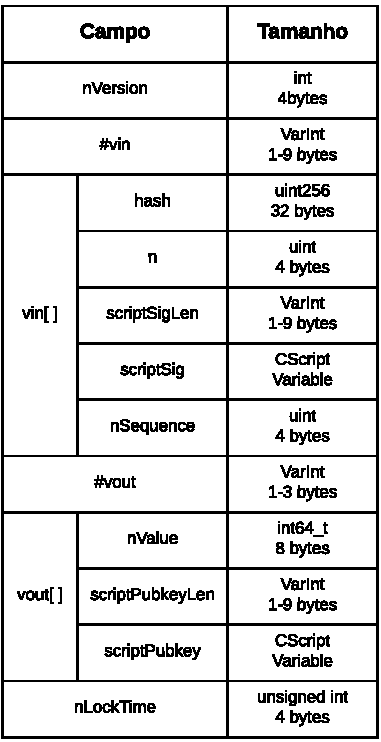
\includegraphics[keepaspectratio=true, scale=0.7]{img/Estrutura_transacao.pdf}
    \caption{Estrutura de uma transação \cite{DevBitKO}}
    \label{fig:Estrutura_transacao}
\end{figure}

Cada transação pode conter mais de um \textit{input} e \textit{output}, e eles são armazenados nos campos \textit{vin}[] e \textit{vout}[] respectivamente. O tamanho desses vetores, que corresponde a quantidade de \textit{inputs} e \textit{outputs} de uma transação, é armazenado nos campos \#vin, para o \textit{vin}[], e \#vout, para o \textit{vout}[].

Cada \textit{output} de transação possui 3 campos: \textit{nValue}, \textit{scriptPubkeyLen} e \textit{scriptPubkey}. O campo \textit{nValue} corresponde uma quantia de Bitcoin em uma unidade chamada Satoshi, essa unidade corresponde a maior divisão que pode-se fazer em uma unidade de Bitcoin que é de 8 casas decimais, ou seja, 1 Satoshi é equivalente 0.00000001\bitcoinA. O \textit{scriptPubkeyLen} armazena o tamanho do \textit{scriptPubkey} que é um script de travamento do UTXO, a linguagem script do bitcoin será apresentada na seção \ref{section:Validando transações}.

Os \textit{outputs} de transação geram pedaços indivisíveis de bitcoin gastáveis chamadas de  \textit{output} de transação não gastos (\textit{Unspent transaction output}) ou UTXO. Ao criar um UTXO ele se torna indivisível, ou seja, seu valor não pode ser divido assim como não se pode dividir uma moeda. Esses UTXO são reconhecidos na rede como quantias de bitcoin que podem ser gastas em uma transação futura.

Os UTXOs são monitorados e armazenados na memória RAM por todos os nós da rede Bitcoin como um conjunto de dados chamado de \textit{pool} UTXO ou UTXO \textit{set}. Sua administrarão é feita automaticamente pela carteira Bitcoin do usuário, assim como sua quantia de Bitcoins. Essa quantia que toda carteira diz possuir não passa de todos os UTXOs associados a chave primaria daquela carteira que estão espalhados no Blockchain. Como efeito disso, não existe um armazenamento de saldo em uma carteira Bitcoin, o que existe na verdade são UTXOs dispersos no blockchain vinculados a uma chave. O conceito de saldo de uma carteira Bitcoin não passa de uma abstração da operação de busca no blockchain e a soma de todas as UTXOs pertencentes a chave primaria de uma carteira.

Os \textit{inputs} de transação são referências aos UTXOs que serão utilizados na transação. Cada \textit{input} possui quatro campos: \textit{hash}, \textit{n}, \textit{coinbaseLen} e \textit{nSequence}. O campo \textit{hash} corresponde ao duplo hash da transacão no blockchain que contém o UTXO que está sendo utilizado no \textit{input}, servindo como referência. O segundo campo armazena a posição do UTXO na transacão anterior, como um index de um vetor. O \textit{scriptSigLen} armazena o tamanho do \textit{scriptSig} que é o script que libera a utilização do UTXO. O \textit{nSequence} armazena o número de sequência do input de transação. Ele foi planejado para a funcionalidade de atualização da transação antes de ser incluída em um bloco através de múltiplas assinaturas, porém essa funcionalidade foi removida para reduzir a complexidade do protocolo.

O \textit{nLockTime} serve como uma trava de tempo para a transação. Assim que o tempo estipulado pelo \textit{nLockTime} for ultrapassado a transação é travada é pode ser incluída em um bloco. Se o valor do \textit{nLockTime} f	or 0 significa que a transação está travada, um valor menor que $5*10^8$ corresponde ao número de blocos que deve-se ter para travar a transação e um valor igual ou acima de $5*10^8$ corresponde ao tempo no formato UNIX que deve-se obter.

\begin{figure}[H]
    \centering
    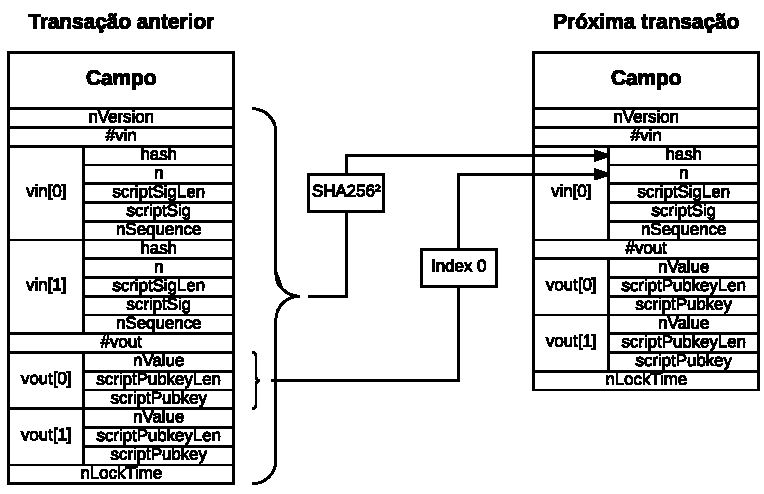
\includegraphics[keepaspectratio=true, scale=0.6]{img/Relacao_inpout_transacao.pdf}
    \caption{Relação entre transação}
    \label{fig:Relacao_inpout_transacao}
\end{figure}

Pode parecer estranha a necessidade de dois \textit{outputs}, mas como um UTXO é indivisível é necessário gerar um troco na transação, e esse segundo output é uma transação de volta para a carteira do usuário com o valor do troco que de ser gerado. Por exemplo,um usuário possui 3 UTXOs de Bitcoin e deseja fazer uma transação de 1 Bitcoin, essa transação precisará consumir todos os 3 UTXOs e irá produzir 2 outpus: uma para o destinatário da transação no valor de 1\bitcoinA{} e outro no valor de 2\bitcoinA{} menos a taxa do minerador como troco de volta para o usuário.

A taxa de transação é paga ao minerador que processou a transação em um bloco como recompensa pelo seu processamento e gasto de energia é são calculadas de acordo com o tamanho da transação em kilobytes, e também servem como desestimuladoras de transações \textit{spam}. As taxas de transação afetam a prioridade do processamento de uma transação, significando uma uma transação com uma taxa alta podem ser incluídas no blockchain mais rapidamente do que uma transação de com uma taxa muito baixa. Um taxa de transação não é obrigatória em uma transação, e as transações sem taxa podem ser processadas.

O valar dessa taxa é calculado através da subtração da soma de todos os \textit{inputs} com a soma de todos os \textit{outputs} ($\sum_{i=0}^{N} \textit{inputs} - \sum_{i=0}^{K} \textit{outputs}$), o valor dessa operação será o valor da taxa. As taxas dadas ao minerador são transferidas para ele através de uma transação criado por ele é inserida no bloco que foi minerado.


\subsection*{Transação coinbase}

A única exceção para essa regra de cadeia de \textit{inputs} e \textit{output} é para um tipo especial de transação chamada \textit{coinbase}. Essa transação é inserida no bloco minerado pelo minerador "vencedor" e tem a finalidade de inserir novos bitcoins na rede, que serão transferidos para o minerador como recompensa por ter minerado o bloco. Como essa novas moedas acabaram de ser criadas essa transação não possui um \textit{input}. A estrutura de uma transação coinbase a apresentada na Figura \ref{fig:Estrutura_coinbase}.

\begin{figure}[H]
    \centering
    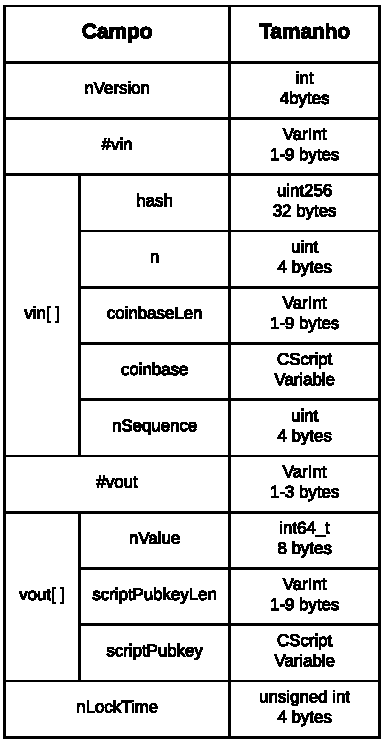
\includegraphics[keepaspectratio=true, scale=0.6]{img/Estrutura_coinbase.pdf}
    \caption{Estrutura de uma transação coinbase \cite{DevBitKO}}
    \label{fig:Estrutura_coinbase}
\end{figure}

A única alteração na transação coinbase são os campos \textit{coinbaseLen}, que armazena o tamanho do segundo campo que é o \textit{coinbase}. O campo \textit{coinbase} funciona como um script de travamanto, por isso é também conhecido por coinbase script. Ele armazena a altura que o blockchain deve ter, a partir do bloco que possui a transação coinbase, para que se possa gastar essas novas moedas. A estrutura do campo \textit{coinbase} é apresentada na Figura \ref{fig:Estrutura_coinbase}. 
 
\begin{figure}[H]
    \centering
    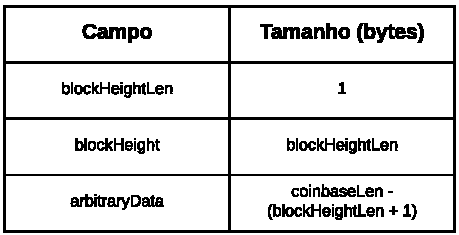
\includegraphics[keepaspectratio=true, scale=0.6]{img/Estrutura_campo_coinbase.pdf}
    \caption{Estrutura do campo coinbase \cite{DevBitKO}}
    \label{fig:Estrutura_campo_coinbase}
\end{figure}

O primeiro campo \textit{blockHeightLen} armazena o tamanho do \textit{blockHeight} que possui a altura do bloco. O dados do campo \textit{arbitraryData} devem ser aleatórios e podem ser utilizados no algoritmo de prova-de-trabalho.


\subsection{Validando transações}
\label{section:Validando transações}
As transações Bitcoin são validadas através de uma linguagem script. São utilizados dois tipos de scripts para a validação: um script de travamento e um de destravamento.

Um script de travamento é uma imposição inserida em um output especificando as condições necessárias para se gastar um UTXO no futuro. O script de travamento é conhecido como \textit{scriptPubKey} pois ele continha uma chave publica ou endereço Bitcoin, porém atualmente utiliza-se uma gama muito maior de possibilidades de script.

%%REVER!!!!!!!!!!!!!! Existem mais que as citadas!!!!!!!!!!!!!!!!!!
Um script de destravamento satisfaz as condições que forem colocas em um UTXO por um script de travamento, permitindo que o UTXO seja gasto. Eles fazem parte de todos os inputs de transação e na maioria das vezes contém uma assinatura digital produzida por uma carteira a partir de sua chave primaria, por isso é conhecido como \textit{scriptSig}, mas nem todos os scripts de destravamento contém uma assinatura digital.

\subsection*{Linguagem Script}  
\label{section:Linguagem Script}
A linguagem script das transações Bitcoin utiliza a notação polonesa invertida, baseada em pilha(\textit{stack}). Uma pilha possui apenas duas operações, empilhar(push) e desempilhar(pop). A operação push insere um item no topo da pilha enquanto a operação pop retira um item do topo da pilha.

Ela não é uma linguagem Turing Completa, o que significa que não se pode criar loops ou algo que de alguma maneira poderia criar um ataque de negação de serviço na rede. Outra forte característica é que ela não exige um monitoramento de estado, ou seja, não existe um estado salvo após a execução do script, toda a informação necessária para executar o script está contida no script. Isso significa que uma transação valida será valida para toda a rede.

Essa linguagem script possui dois tipos de dados, constantes de dados(números) e operadores, e executa-os da esquerda para direita. Os operadores podem desempilhar(pop) constantes de dados, opera-las e empilha-las(push) novamente. Enquanto uma constantes de dados são sempre empilhadas(push).

Atualmente existem cinco tipos padrões de scripts de transação: \textit{pay-to-public-key-hash}(P2PKH), \textit{Pay-to-Public-Key}(P2PK), \textit{multi-signature}, \textit{Pay-to-script-hash}(P2SH) e \textit{data output} (OP\_RETURN). Todos esse script serão abordados a seguir.

\subsection*{Pay-to-Public-Key-Hash}
O script de transação Pay-to-Public-Key-Hash(P2PKH) utiliza um script de travamento que disponibiliza um \textit{output} para um endereço Bitcoin, que é o hash da chave pública da carteira. Esse \textit{output} pode ser destravado ao se apresentar a chave pública e a assinatura digital criada pela chave privada correspondente.

Para melhor entender o funcionamento desse script vamos supor que Bob deseja fazer uma transação de uma quantia de bitcoins que existe em sua carteira para a carteira de um café de sua cidade. O script de travamento do UTXO que será inserido no \textit{input} dessa transação possui a seguinte forma.


\begin{figure}[H]
    \centering
    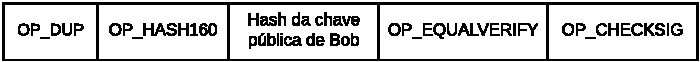
\includegraphics[keepaspectratio=true, scale=0.7]{img/P2PHKH_script_travamento.pdf}
    \caption{Exemplo de script de travamento P2PHKH}
    \label{fig:P2PKH_Travamento}
\end{figure}

O script de destravamento que satisfaz o script de travamento P2PKH é o seguinte.

\begin{figure}[H]
    \centering
    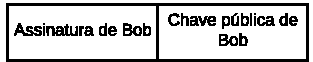
\includegraphics[keepaspectratio=true, scale=0.8]{img/P2PHKH_script_destravamento.pdf}
    \caption{Exemplo de script de destravamento P2PHKH}
    \label{fig:P2PKH_Destravamento}
\end{figure}

Ao juntarmos os scripts de travamento e destravamento temos o seguinte script de validação.

\begin{figure}[H]
    \centering
    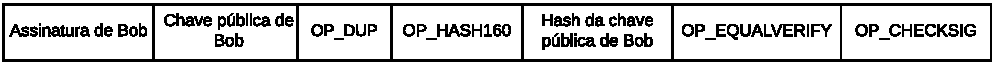
\includegraphics[keepaspectratio=true, scale=0.47]{img/P2PHKH_script_validacao.pdf}
    \caption{Exemplo de script de validação P2PHKH}
    \label{fig:P2PKH_Validacao}
\end{figure}

Esse script de validação será executado na seguinte forma.


\begin{enumerate}
\item A assinatura de Bob é inserido no topo da pilha;
\item A chave pública de Bob é inserida no topo da pilha, acima da assinatura de Bob;
\item O operador OP\_DUP é executado, ele duplica o dado que está no topo da pilha e o resultado é empilhado;
\item O operador OP\_HASH160 é executado, ele aplica o hash RIPEMD160(SHA256) no dado que está no topo da pilha e empilha o resultado;
\item O hash da chave pública (enderećo Bitcoin) de Bob é empilhado;
\item A operaćão OP\_EQUALVERIFY é executada, essa operação retira da pilha dois dados mais próximos ao topo e os compara. No caso do P2PKH será comparado o hash da chave pública de Bob empilhada em 5 com o calculada em 4. Se os hashs forem iguais, ambos são removidos e a operação continua;
\item É executada a operação OP\_CHECKSIG, ela verifica se a assinatura de Bob combina com a chave pública fornecida, se a assinatura combinar com a chave pública fornecida a operação empilha o valor TRUE na pilha. As assinaturas no Bitcoin utilizam o Algoritmo de Assinatura Digital de Curvas Elípticas(ECDSA).
\end{enumerate}

\subsection*{Pay-to-Public-Key}
O script Pay-to-Public-Key(P2PK) utiliza a chave pública no script de travamento, ao invés do hash da chave pública como no P2PKH. 

O script de travamento do P2PK possui a seguinte forma.
 
\begin{figure}[H]
    \centering
    
\includegraphics[keepaspectratio=true, scale=0.8]{img/P2PK_script_travamento.pdf}
    \caption{Exemplo de script de travamento P2PK}
    \label{fig:P2PK_Travamento}
\end{figure}


O script de destravamento que deve ser apresentado para se utilizar o UTXO é apenas uma assinatura a partir da chave privada de Bob.

\begin{figure}[H]
    \centering
    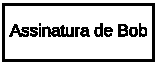
\includegraphics[keepaspectratio=true, scale=0.8]{img/P2PK_script_destravamento.pdf}
    \caption{Exemplo de script de destravamento P2PK}
    \label{fig:P2PK_Destravamento}
\end{figure}

Ao juntarmos os scripts de travamento e destravamento temos o seguinte script de validação.

\begin{figure}[H]
    \centering
    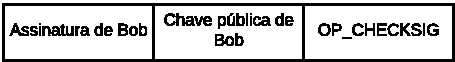
\includegraphics[keepaspectratio=true, scale=0.8]{img/P2PK_script_validacao.pdf}
    \caption{Exemplo de script de validação P2PK}
    \label{fig:P2PK_Validacao}
\end{figure}

Esse script é bem mais simples que o P2PKH, porém o seu script de travamento ocupa muito mais espaço já que a chave pública é maior que seu hash, o que dificulta seu uso. O script P2PK é mais utilizado hoje por softwares de mineração mais antigos que não foram atualizados para utilizarem o P2PHK.

\subsection*{Multi-signature}
\label{sec:Multi-signature}
Esse script de transação define uma condição onde N chaves públicas são registradas no script e pelo menos M dessas chaves devem ser fornecidas para a liberação de tal UTXO. Essa condição é conhecida como um esquema M-de-N, onde N é o número total de chaves e M é o número de assinaturas necessárias para a liberação do UTXO.

O script de travamento de um script Multi-signature é da seguinte forma.

\begin{figure}[H]
    \centering
    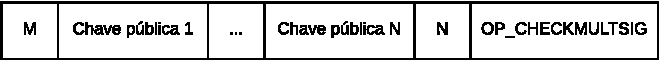
\includegraphics[keepaspectratio=true, scale=0.75]{img/Multsig_script_travamento.pdf}
    \caption{Exemplo de script de travamento Multi-signature}
    \label{fig:Multi-signature_Travamento}
\end{figure}

O script de destravamento Multi-signature deve apresentar M-de-N assinaturas.

\begin{figure}[H]
    \centering
    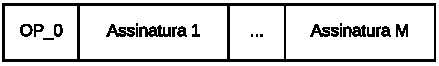
\includegraphics[keepaspectratio=true, scale=0.75]{img/Multsig_script_destravamento.pdf}
    \caption{Exemplo de script de destravamento Multi-signature}
    \label{fig:Multi-signature_Destravamento}
\end{figure}

Ao juntarmos os scripts de travamento e destravamento temos o seguinte script de validação.

\begin{figure}[H]
    \centering
    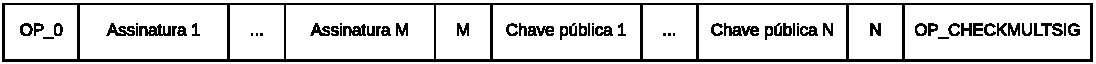
\includegraphics[keepaspectratio=true, scale=0.45]{img/Multsig_script_validacao.pdf}
    \caption{Exemplo de script de validação Multi-signature}
    \label{fig:Multi-signature_validacao}
\end{figure}

Os scripts Multi-signature são os exemplos mais comuns das avançadas capacidades do script Bitcoin e são uma funcionalidade muito poderosa. Como é necessário mais de uma assinatura para liberação dos fundos, um esquema de múltiplas assinaturas como esse oferece um controle de governança corporativa e protege os fundos contra roubo, desvios ou perdas.

Apesar de todas as vantagens dos scripts Multi-signature suas desvantagens acabam inviabilizando seu uso. As transações Multi-signature são bem maiores que as transações de pagamento simples, pois elas contém chaves públicas muito longas. O fardo de uma transação extra-grande carregado pelo sistema teria que ser compensado com uma taxa de transação bem maior que as pagas pelas transações de menor tamanho, e além disso esses scripts extra-grandes teriam que ser carregados no \textit{pool} UTXO de cada nó da rede até que seja gasto. Outro grande problema e talvez o maior é que para cada transação desse tipo teriamos um script de transação customizado, logo teríamos que ter uma carteira que possibilita a criação de tais scripts customizados e cada usuário teria que entender como criar transações com scripts customizados. Para resolver o problema dessa dificuldades práticas e fazer a utilização de scripts complexos tão fácil quanto o P2PKH foi desenvolvido o script Pay-to-Script-Hash(P2SH).

\subsection*{Pay-to-Script-Hash}

Nos scripts Pay-to-Script-Hash(P2SH) é utilizado o hash criptográfico do script de travamento apresentado em \ref{sec:Multi-signature}, ou seja, o script de travamento complexo e substituído pela sua impressão digital. Esse hash criptográfico codificado na Base58Check corresponde ao endereço P2PH, assim como o hash da chave pública corresponde ao endereço Bitcoin. Com o endereco P2PH resolvemos todos os proplemas apresentados em \ref{sec:Multi-signature}. Agora basta fornecer o endereco P2SH para conseguir efetuar uma transacao, um processo simples, similar ao executado no script P2PKH.

Nas transações P2SH o script de travamento é o endereço P2PH e o script de travamento do Multi-signature aqui é conhecido como script de resgate(\textit{redeem script}), pois ele deve ser apresentado na hora do resgate dos UTXOs. O script de destravamento deve conter as assinaturas necessárias para desbloquear os UTXOs, a condição M-de-N também devem ser satisfeita no P2SH. As Tabelas \ref{table:Multi-signature_sem_P2SH} e \ref{table:Multi-signature_com_P2SH} apresentam os scripts no esquema de Mult-signature sem o P2SH e com o P2SH respectivamente.

\begin{table}[H]
\centering
\caption{Multi-signature sem P2SH}
\label{table:Multi-signature_sem_P2SH}
\begin{tabular}{|l|l|}
\hline
Script de travamento    & M PK1 ... PKn N CHECKMULTISIG \\ \hline
Script de destravamento & Ass1 ... Assn                  \\ \hline
\end{tabular}
\end{table}

\begin{table}[H]
\centering
\caption{Multi-signature com P2SH}
\label{table:Multi-signature_com_P2SH}
\begin{tabular}{|l|l|}
\hline
Script de resgate       & M PK1 ... PKn N CHECKMULTISIG                                                                      \\ \hline
Script de travamento    & \begin{tabular}[c]{@{}l@{}}OP\_HASH160 \textless endereço P2SH\textgreater \\ OP\_EQUALVERIFY\end{tabular} \\ \hline
Script de destravamento & Ass1 ... Assn                                                                                              \\ \hline
\end{tabular}
\end{table}

\subsection*{Data Recording Output (OP\_RETURN)}

Todas as transações da rede Bitcoin são armazenas em um "banco de dados" distribuído chamado Blockchain, o funcionamento desse sistema será explicado mais adiante. Esse sistema potencial muito mais amplo do que apenas pagamentos, muitos desenvolvedores tentaram utilizar da segurança e resiliência do Blockchain para aplicações como cartórios digitais, certificados de ações e contratos \textit{smart}. As primeiras tentativos surgiram ao tentar criar \textit{outputs} de transação que registravam dados no Blockchain.

Quando a ideia de utilizar o Blockchain do Bitcoin  consideram esse uso abusivo, enquanto outros acreditaram que isso mostrava a enorme capacidade dessa tecnologia. Os que eram contra argumentavam que isso causaria um "inchaço" no blockchain", trazendo uma carga par os nós que armazenam o blockchain em disco. Além disso, esse processo criaria  falsas transações já que utilizam o campo de endereço do destinatário para armazenar dados, fazendo com que o UTXO jamais seja gasto. Essas transações que não podem ser gastas jamais seriam removidas do \textit{pool} UTXO fazendo-o crescer infinitamente. 

%Review
Para resolver esse problema na versão BitcoinCore 0.9.0 foi introduzido o operador OP\_return, esse operador permitia que fosse adicionado 40 bytes de não-pagamento em um \textit{output} de transação, na versão BitconCore 0.12.0 esse limite foi aumentado para 83 bytes. Esse operador cria \textit{outputs} que são comprovadamente não gastáveis que não precisam ser registrados no \textit{pool} UTXO.


\subsection{Blockchain}
O blockchain funciona como uma de registros público distribuído e compartilhado. No bitcoin o blockchain funciona como um livro-razão onde são armazenadas todas as transações já feitas. Seu principal proposito é garantir uma ordem cronológica das transações e prevenir o problema de gasto duplo (double spending), apresentado por Hal Finney em seu whitepaper intitulado Digital Cash \& Privacy. 

A estrutura do blockchain é vista como um estrutura ordenada de blocos de dados com cada bloco sendo identificado pelo seu hash (SHA256). Cada bloco contém uma referência ao bloco anterior (bloco pai) em seu cabeçalho, essa referência corresponde ao identificador do bloco anterior. Isso empoe uma ordem cronológica nos blocos e por consequência nas transações, já que não é possível criar o hash de um bloco que ainda não existe no blockchain. O único bloco que não possui a referência para seu bloco pai é o bloco gênese, pelo fato de ser o primeiro bloco do blockchain. 

O bloco gênese é o ancestral comum de todos os blocos do blockchain. Esse bloco gênese está estaticamente codificado no cliente bitcoin fazendo com que todo nó comece com o bloco gênese em seu blockchain. Como o nó conhece todos os dados da estrutura do bloco gênese, ele contém um ponto de partida do blockchain seguro, a partir do qual pode montar uma blockchain de confiança. 

Devido cronologia existente entre os blocos podemos abstrair o blockchain como um empilhamento de blocos de dados, com cada  novo bloco gerado sendo empilhado sobre o bloco mais recente do blockchain. Essa visualização de blocos empilhados possibilita a utilização de termos como "altura", para se referir a posição de um bloco em relação ao primeiro bloco do blockchain (Bloco gênese), e "topo", para se referir ao bloco mais recente do blockchain. 

Como cada bloco possui a o hash de seu bloco pai em seu cabeçalho isso irá influenciar no seu hash, assim, se ocorrer uma mudança em um bloco isso afetará seu hash que também afetará os blocos acima causando um efeito dominó. Esse efeito dominó garante a  que um bloco que tenha algumas gerações o sucedendo não possa ser alterando, a não ser que haja um calculo forçado do hash de todos os blocos subsequentes. Essa é uma das características chave para a segurança do blockchain, pois a mudança de um bloco que já possui uma certa profundidade exigira um processo computacional enorme.

Os blocos também possuem a solução para o algoritmo de prova de trabalho. O trabalho computacional envolvido na solução do problema de prova de trabalho é utilizado como um esquema de votação entre os nós da rede para que eles concordem com a versão do blockchain. No geral, os nós concordam a com a versão do blockchain que envolva o maior poder computacional utilizado para ser criado.

Como os nós mineradores da rede competem na solução de prova de trabalho para incluir um bloco no blockchain, existe a possibilidade de dois blocos serem minerados ao mesmo tempo, causando um bifurcação no blockchain visto pela rede. Nesse caso os nós irão aceitar o bloco que receberem primeiro e continuar a construir o blockchain a partir daquele bloco. Assim que um novo bloco for adicionado a uma das bifurcações, aquela com maior altura será considerado o blockchain válido e as transações do bloco descartado serão adicionadas ao pool de transações.



\subsection*{Estrutura de um bloco}
Cada bloco no blockchain do Bitcoin é composto por um cabeçalho e um payload e sua estrutura é apresentada na Tabela \ref{table:estrutura_bloco}. O cabeçalho corresponde aos 6 primeiros campos e o payload aos dois últimos.

\begin{table}[H]
\centering
\caption{Estrutura de um bloco \cite{DevBitKO}}
\label{table:estrutura_bloco}
\begin{tabular}{|l|c|}
\hline
\multicolumn{1}{|c|}{\textbf{Campo}} & \textbf{Tamanho}                                                 \\ \hline
\textit{nVersion}                             & \begin{tabular}[c]{@{}c@{}}int\\ (4 bytes)\end{tabular}          \\ \hline
\textit{HashPrevBlock}                        & \begin{tabular}[c]{@{}c@{}}uint256\\ (32 bytes)\end{tabular}     \\ \hline
\textit{HashMerkleRoot}                       & \begin{tabular}[c]{@{}c@{}}uint256\\ (32 bytes)\end{tabular}     \\ \hline
\textit{nTime}                                & \begin{tabular}[c]{@{}c@{}}unsigned int\\ (4 bytes)\end{tabular} \\ \hline
\textit{nBits}                                & \begin{tabular}[c]{@{}c@{}}unsigned int\\ (4 bytes)\end{tabular} \\ \hline
\textit{nNonce}                               & \begin{tabular}[c]{@{}c@{}}unsigned int\\ (4 bytes)\end{tabular} \\ \hline
\textit{\#vtx}                                & \begin{tabular}[c]{@{}c@{}}VarInt\\ (1-9 bytes)\end{tabular}     \\ \hline
\textit{vtx}{[}{]}                            & Variable                                                         \\ \hline
\end{tabular}
\end{table}

O campo \textit{nVersion} armazena o número de versão como referências as atualizações de software/protocolo. O segundo campo \textit{HashPrevBlock} corresponde ao duplo hash dos dados concatenados do cabeçalho bloco anterior (bloco pai), que é o identificador primário do bloco, como apresentado na Figura \ref{fig:Ref_blocos}. Essa ligação entre os blocos é uma das características chaves que garante a segurança e resiliência do Blockchain e foi explicada do início dessa seção. O \textit{HashMerkleRoot} armazena o hash da raiz da árvore de Merkle das transações desse bloco. Os campos \textit{nTime} e \textit{nBits} correspondem ao tempo aproximado no formato UNIX em que o bloco foi criado e a dificuldade do algoritmo de prova-de-trabalho do bloco. O \textit{nNonce} é uma sequência de bit aleatória e é utilizado como fonte de aleatoriedade para o algoritmo de prova-de-trabalho. Entretanto como o \textit{nNonce} possui um tamanho muito pequeno ele não prove uma variância significante, devido a isso existem outras fontes que serão apresentadas com mais detalhes na seção \ref{}.

No payload temos os campos \textit{\#vtx} que armazena a quantidade de transações que o campo \textit{vtx}[] possui. O campo \textit{vtx}[] funciona como um vetor de transações. A estrutura de uma transações foi apresentada na seção \ref{section:Transações na rede Bitcoin}.

\begin{figure}[H]
    \centering
    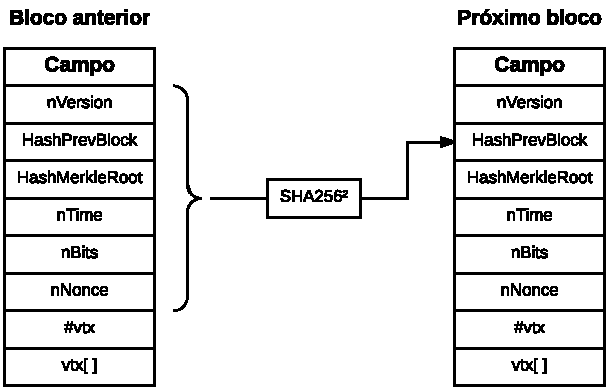
\includegraphics[keepaspectratio=true, scale=0.6]{img/Referencia_entre_blocos.pdf}
    \caption{Referência entre blocos}
    \label{fig:Ref_blocos}
\end{figure}

Perceba que o não está incluído na estrutura de dados do bloco, nem quando o bloco é transmitido na rede e nem quando ele é armazenado no blockchain. O hash deve ser calculado por cada nó assim que o bloco é recebido, e pode ser armazenado em uma tabela separada como parte dos metadados do bloco para facilitar a indexação e uma coleta mais rápida dos blocos em disco. 

%\subsection*{Árvode de Merkle}

%\subsection*{Filtros Bloom}
 
\subsection{Mineração} 
A mineração é um dos processos que torna o bitcoin especial. Ele é o que garante a segurança da rede bitcoin e permite a existência de um consenso em toda a rede sem a necessidade de uma autoridade central. Ela também protege a rede bitcoin contra transações fraudulentas e o problema de gasto duplo (\textit{double spending}).

Esse processo de mineração é o responsável pela criação de novos blocos que serão inseridos no blockcahin, e ele é executados pelos nós mineradores da rede. Esses nós apuram e validam todas as transações que serão inseridas no bloco, e cada novo bloco é "minerado" em média a cada 10 minutos.

Além de gerar novos blocos a mineração também é responsável por inserir novas moedas na rede. Essas moedas são geradas através da transação coinbase para minerador que gerou o novo bloco como recompensa. Essa recompensa aos minerados é o que gera a oferta monetária do bitcoin, semelhante à maneira que um banco central emite dinheiro através da impressão de novas cédulas. A quantidade de bitoins de uma transação coinbase diminuiu pela metade a cada 210.000 blocos minerados (em média a cada 4 anos). No começo do bitcoin, em janeiro de 2009, uma transação coinbase continha 50 bitcoins, essa quantidade caiu para 25 em novembro de 2012 e em 2016 caiu para 12,5. Com base nessa fórmula, a remuneração do bitcoin diminuirá exponencialmente até aproximadamente o ano de 2140, quando todos os 20,99999998 milhões de bitcoins já estarão em circulação.

\subsection*{O consenso descentralizado}
Todos os modelos de pagamento tradicionais utilizam uma autoridade central que forneça um serviço de compensação, verificação e registro de todas as transações. O bitcoin não possui uma autoridade central para verificar e compensar as transações, ele utiliza o blockchain como um registro público de todas as transações da rede e que todos o participantes confiam e aceitam com o registro oficial de posse dos bitcoins.

A principal invenção de Satoshi Nakamoto é o mecanismo descentralizado utilizado para geral o consenso emergente. Diz-se emergente porque o consenso não é atingido de maneira explícita, não existe uma eleição ou um momento exato fixo no qual o consenso é atingido. Ao invés disso o consenso emerge da interação assíncrona de vários nós independentes, com todos seguindo regras simples.

Esse consenso descentralizado emerge da interação de quatro processos que ocorrem independentemente nós nos da rede.

\begin{itemize}
  \item Verificação independente de cada transação pelos Full nodes baseado em uma extensa lista de critérios;
  \item Agregação independente das transações em novos blocos pelos nós mineradores, associado a prova de que um processo computacional foi realizado através do algoritmo prova-de-trabalho;
  \item Verificação independente dos novos blocos por cada nó;
  \item Seleção independente por cada nó do blockchain com o maior poder computacional acumulado demostrado através do algoritmo de prova de trabalho.
\end{itemize}  

\subsection*{Verificação independente das transações}
Vimos em \ref{section:Transações na rede Bitcoin} que uma transação após ser criada é propagada na rede através de nós da rede bitcoin. Porém antes de propagar uma transação para os seus vizinhos o nó deve primeiro validá-la e somente propagar as transações válidas e descartar as transações inválidas.

Cada nó verifica as transações de acordo com uma lista de verificações com vários critérios:

\begin{itemize}
\item A sintaxe da transação e estrutura de dados devem estar corretas;
\item A lista de \textit{inputs} e \textit{outputs} não devem estar vazias;
\item O tamanho da transação em bytes deve ser menor que \texttt{MAX\_BLOCK\_SIZE};
\item O número de operações de assinatura contidas na transação é menor que o limite de operações de assinatura;
\item O scriptSig (script de destravamento) só pode empurrar números para a pilha, e o scriptPubKey (script de destravamento) deve coincidir com as formas isStandard;
\item Deve existir transações correspondentes no pool ou em um bloco no blockchain;
\item Para cada \textit{input}, se o \textit{output} referenciado existir em qualquer outra transação no pool, a transação deve ser rejeitada;
\item Para cada \textit{input}, buscar no blockchain e no pool de transações pelo \textit{output} de transação referenciado. Se o \textit{output} de transação estiver faltando para qualquer \textit{input} essa será uma transação órfã. Ela deve ser adicionada ao pool de transações órfãs, se uma transação correspondente já não estiver no pool;
\item Para cada \textit{input}, se o \textit{output} de transação referenciado for um \textit{output coinbase} ele deve respeitar o valor \texttt{COINBASE\_MATURITY} confirmações;
\item Para cada \textit{input}, o \textit{output} referenciado deve existir e não pode ter sido gasto previamente;
\item Ao usar os \textit{outputs} de transações referenciados para administrar os valores de \textit{input}, deve-se verificar se cada valor de \textit{input}, assim como a soma, estão na faixa permitida de valores (menor que 21 milhões de bitcoin e maior que 0);
\item Rejeitar se a soma dos \textit{inputs} for menor que a soma dos \textit{outputs};
\item rejeitar se a taxa de transação for muito baixa para entrar em um bloco vazio;
\item Os scriptSig (script de destravamento) para cada \textit{input} devem ser validados em relação aos scriptPubKey (script de destravamento) dos \textit{outputs} correspondentes.
\end{itemize}

Essas condições podem ser vistas nas funções AcceptToMemoryPool, CheckTransaction e CheckInputs no cliente Bitcoin. Elas condições podem mudar ao longo do tempo para lidar com novos tipos de ataques de negação de serviço e para incluir novos tipos de transações.

\subsection*{Inserindo transações em um bloco}
Vimos em \ref{section:Tipos de nós} que existem dois tipos de mineradores, os mineradores solo e os mineradores pool. Os mineradores pool são aqueles que participam de um pool de mineração. Esses pools de mineração são utilizados pelos mineradores que não possuem um poder computacional grande suficiente e para ter alguma chance de minerar um bloco eles se juntam nesses pools para agrupar seu poder computacional e dividir a recompensa entre eles de acordo com sua contribuição para encontrar o bloco. Não iremos focar nos minerados pool, analisaremos o processo pelos minerados solo.


\section{Conclusion}
The conclusion goes here.




% conference papers do not normally have an appendix



% use section* for acknowledgment
\ifCLASSOPTIONcompsoc
  % The Computer Society usually uses the plural form
  \section*{Acknowledgments}
\else
  % regular IEEE prefers the singular form
  \section*{Acknowledgment}
\fi


The authors would like to thank...





% trigger a \newpage just before the given reference
% number - used to balance the columns on the last page
% adjust value as needed - may need to be readjusted if
% the document is modified later
%\IEEEtriggeratref{8}
% The "triggered" command can be changed if desired:
%\IEEEtriggercmd{\enlargethispage{-5in}}

% references section

% can use a bibliography generated by BibTeX as a .bbl file
% BibTeX documentation can be easily obtained at:
% http://mirror.ctan.org/biblio/bibtex/contrib/doc/
% The IEEEtran BibTeX style support page is at:
% http://www.michaelshell.org/tex/ieeetran/bibtex/
%\bibliographystyle{IEEEtran}
% argument is your BibTeX string definitions and bibliography database(s)
%\bibliography{IEEEabrv,../bib/paper}
%
% <OR> manually copy in the resultant .bbl file
% set second argument of \begin to the number of references
% (used to reserve space for the reference number labels box)
%\begin{thebibliography}{1}

%\bibitem{IEEEhowto:kopka}
%H.~Kopka and P.~W. Daly, \emph{A Guide to \LaTeX}, 3rd~ed.\hskip 1em plus
%  0.5em minus 0.4em\relax Harlow, England: Addison-Wesley, 1999.

%\end{thebibliography}

\bibliographystyle{abbrv}
\bibliography{Blockchain}


% that's all folks
\end{document}


